\begin{flushright} {\tiny {\color{gray} python\_codes/fieldstone\_100/text.tex}} \end{flushright}

\lstinputlisting[language=bash,basicstyle=\small]{python_codes/fieldstone_100/keywords}

\begin{center}
Code at \url{https://github.com/cedrict/fieldstone/tree/master/python_codes/fieldstone_100}
\end{center}

\par\noindent\rule{\textwidth}{0.4pt}

{\sl This fieldstone was developed in collaboration with B. Root}. \index{contributors}{B. Root}

\par\noindent\rule{\textwidth}{0.4pt}
%%%%%%%%%%%%%%%%%%%%%%%%%%%%%%%%%%%%%%%%%%%%%%%%%%%%%%%%%%%%%%%%%%%%%%%%%%%%%%%%%%%%%%%%%%%%%%

Very high resolution topography datasets of Mars are available at 
\url{https://astrogeology.usgs.gov/search/details/Mars/GlobalSurveyor/MOLA/Mars_MGS_MOLA_DEM_mosaic_global_463m/cub}.
However the data format is not very convenient so Bart Root 
helped me out and exported the data to ascii format.

The file {\filenamefont MOLA\_1deg.txt} counts 64,800 lines, 
i.e. 360x180 points. Longitude values range from  
0.5 to 359.5 and latitudes from -89.5 to +89.5. 

The file {\filenamefont MOLA\_0.5deg.txt} counts 4 times as many lines, 
i.e. 720x360 points=259,200. Longitude values range from  
0.25 to 359.75 and latitudes from -89.75 to +89.75. 

The file {\filenamefont MOLA\_0.25deg.txt} counts 4 times as many lines, 
i.e. 1,036,800 points.

The file {\filenamefont MOLA\_0.0625deg.txt} counts 16 times as many lines, 
i.e. 16,588,800 points.

We follow a similar approach as in \stone 97 and use the data to produce 
two vtu files, one on a 2D plane, one on a 3D sphere:

\begin{center}
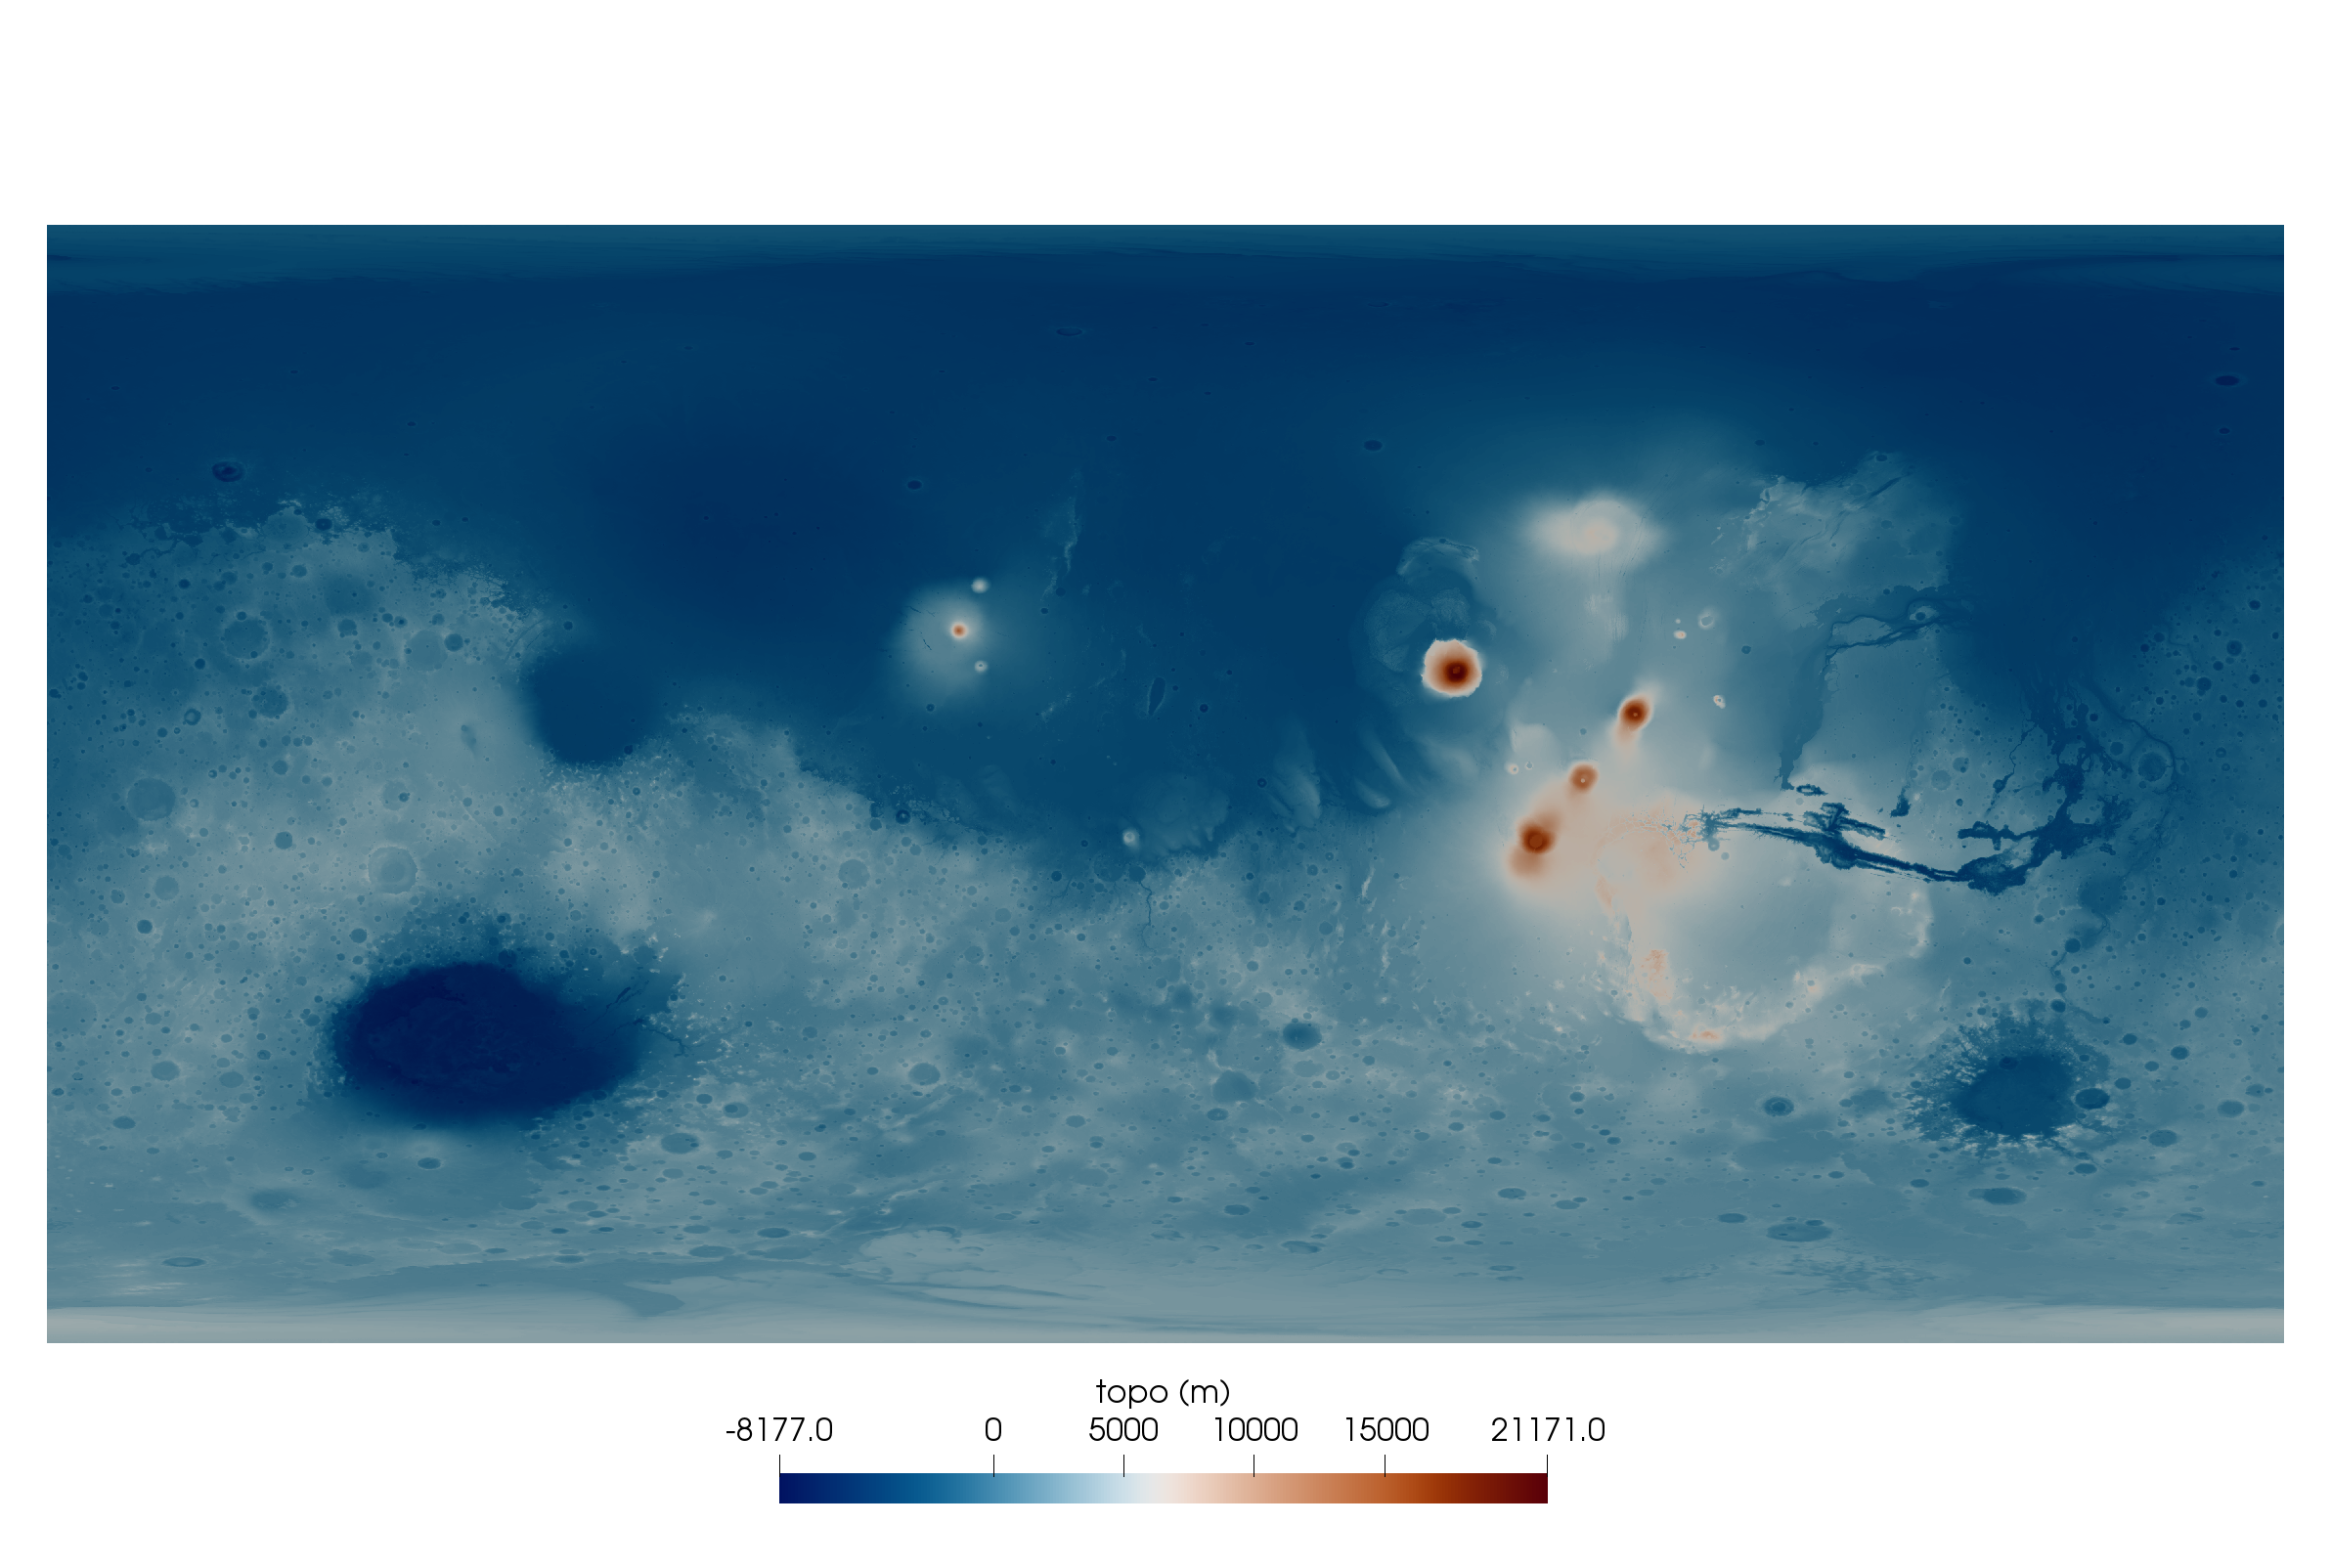
\includegraphics[width=15cm]{python_codes/fieldstone_100/images/topo2D_a}\\

\includegraphics[width=5cm]{python_codes/fieldstone_100/images/topo2D_b}

\includegraphics[width=5cm]{python_codes/fieldstone_100/images/topo2D_c}
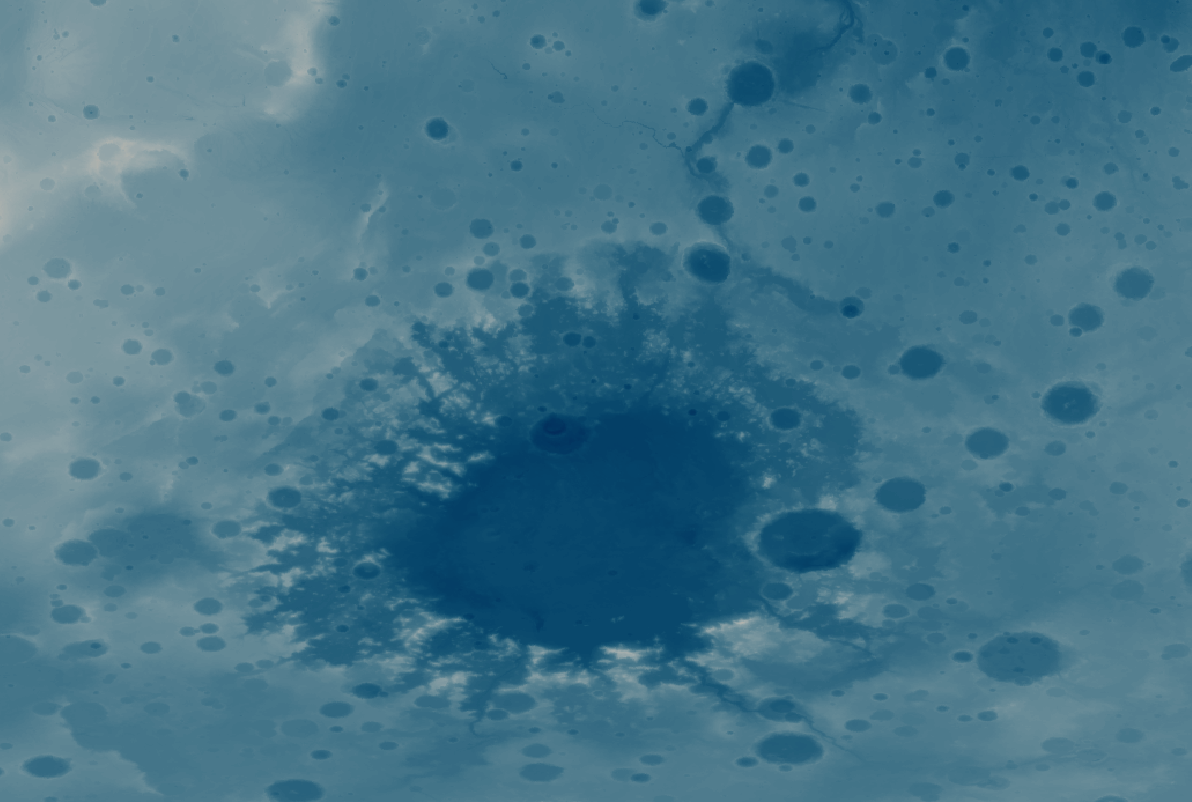
\includegraphics[width=5cm]{python_codes/fieldstone_100/images/topo2D_d}\\
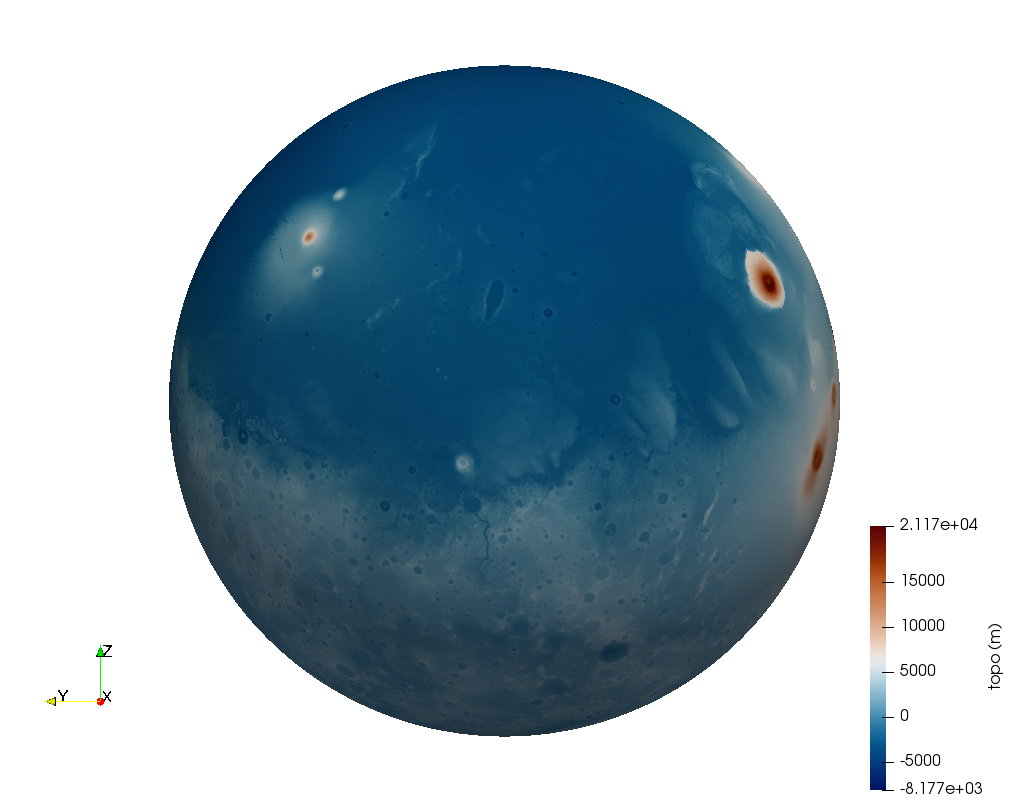
\includegraphics[width=5cm]{python_codes/fieldstone_100/images/topo3D_1}
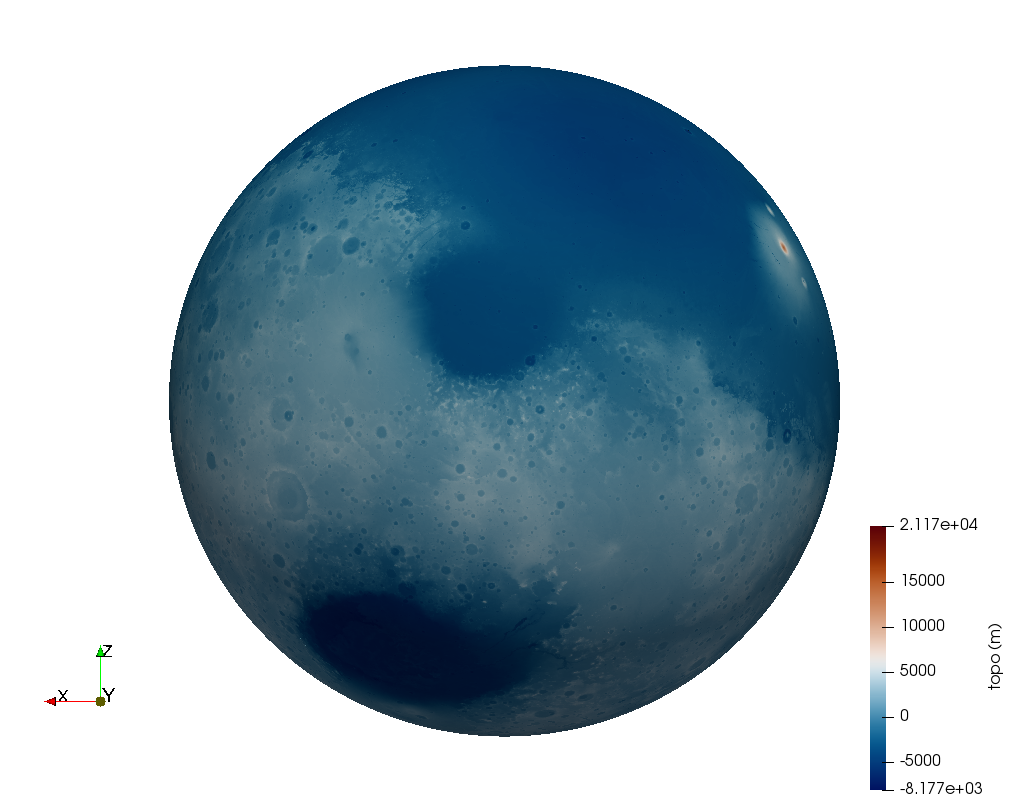
\includegraphics[width=5cm]{python_codes/fieldstone_100/images/topo3D_4}
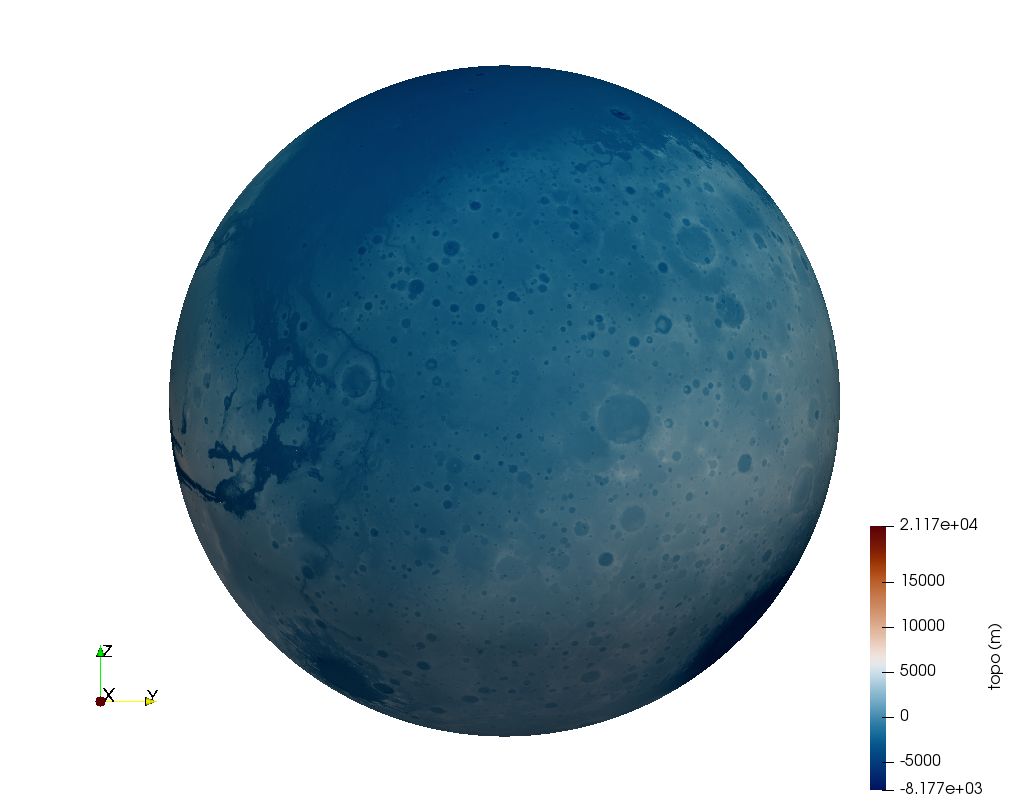
\includegraphics[width=5cm]{python_codes/fieldstone_100/images/topo3D_2}\\
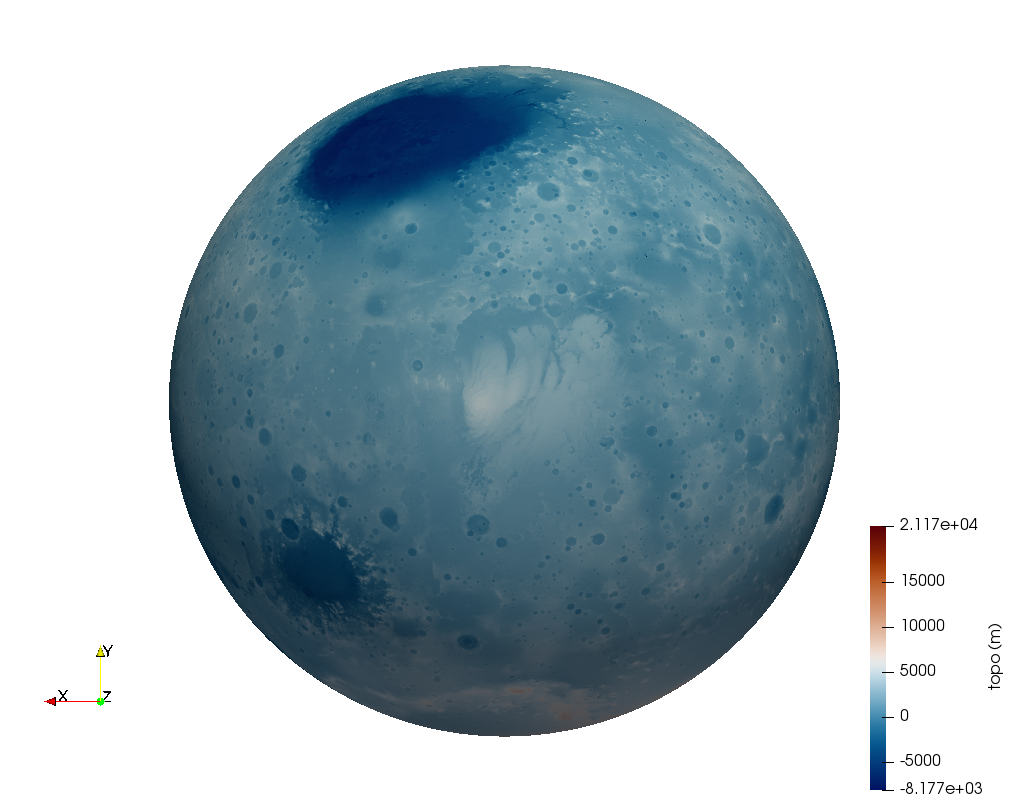
\includegraphics[width=5cm]{python_codes/fieldstone_100/images/topo3D_5}
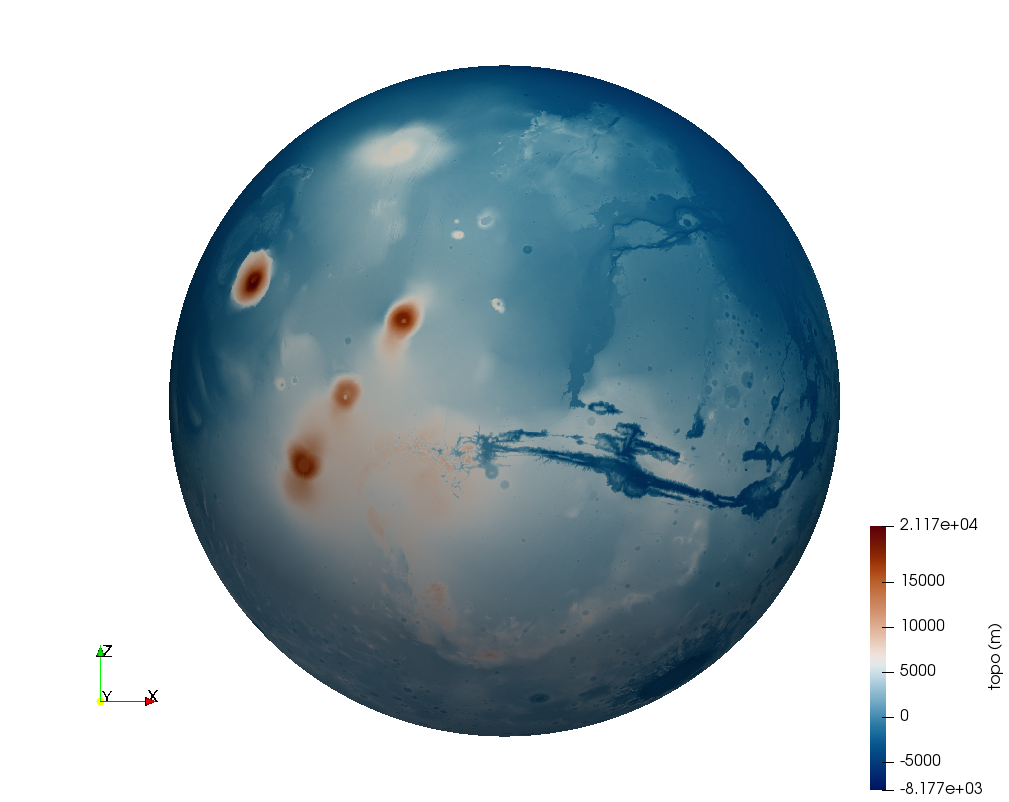
\includegraphics[width=5cm]{python_codes/fieldstone_100/images/topo3D_3}
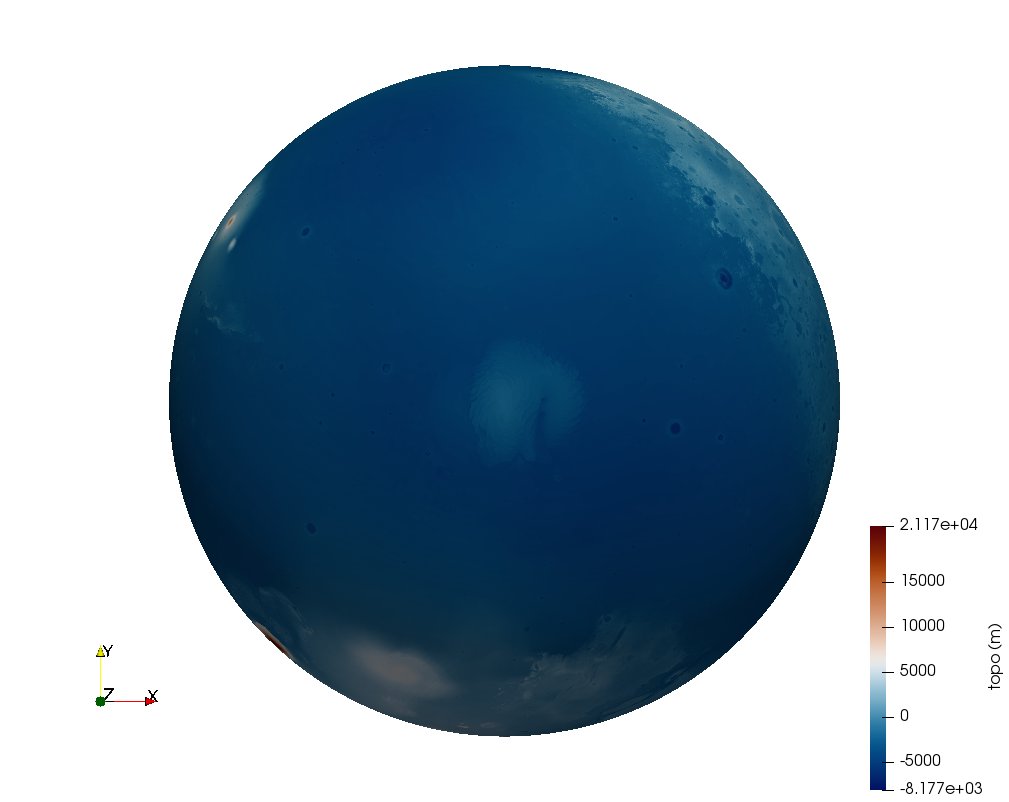
\includegraphics[width=5cm]{python_codes/fieldstone_100/images/topo3D_6}\\
{\captionfont Based on the 0.0625degree resolution file.}
\end{center}

Note that the files corresponding to 1/2, 1/4, and 1/16 of degree are not on github since they are quite large. 
Please contact me.

%-------------------------------------------------------------------
\subsection*{Using the topography to compute its gravity signal}

Each cell is characterised by a min/max latitude, longitude. We can convert these to 
spherical coordinates with $\phi$ being the longitude and $\theta$ being the colatitude.
The topography is given with respect to the Mars radius $R_{mars}$. Since the minimum 
of the topography is about $-7.7~\si{\km}$ we define the inner radius of the hollow planet 
as $R_{min}=R_{mars}-t$ with $t=8~\si{\km}$. The topography associated to the cell is the one in its middle
so we define $R_{max}=R_{mars}+h$ where $h$ is the topography in the cell middle. 
Each cell then has a volume
\begin{eqnarray}
V
&=&
\int_{\phi_{min}}^{\phi_{max}}
\int_{\theta_{min}}^{\theta_{max}}
\int_{R_{min}}^{R_{max}}
dV \nn\\
&=&
\int_{\phi_{min}}^{\phi_{max}}
\int_{\theta_{min}}^{\theta_{max}}
\int_{R_{min}}^{R_{max}}
r^2 \sin\theta dr d\theta d\phi \nn\\
&=&
\int_{\phi_{min}}^{\phi_{max}} d\phi \cdot
\int_{\theta_{min}}^{\theta_{max}} \sin\theta d\theta \cdot 
\int_{R_{min}}^{R_{max}} r^2 dr\nn\\
&=&
(\phi_{max} -\phi_{min})
(\cos \theta_{min} -\cos\theta_{max})
\frac13 (R_{max}^3-R_{min}^3)
\end{eqnarray}
We will assume for simplicity that the upper crust has a constant density $\rho_c$. 

The last step is to define the center of the cell. The $\theta_c$ and $\phi_c$ 
coordinates of the cell middle point are trivial, they are those from the 
topography file. In the radial direction, we shall simply take
\[
r_c(\theta_c,\phi_c)=\frac12( R_{min}+R_{max})=\frac12 (R_{mars}+h(\theta_c,\phi_c)+R_{mars}-t)= R_{mars} + \frac12[h(\theta_c,\phi_c)-t]
\]
We can now proceed to compute the gravity field(s) 
resulting from this thin crustal layer at a point $\vec{r}=(x,y,z)$, as 
explained in Section~\ref{}.


On Mars, 1degree = $2\pi R_{mars}/360 \simeq 59~\si{\km}$, so that the highest resolution
corresponds to a cell of side $\sim 3.7~\si{\km}$!


idea/todo: divide columns radially so as to obtain almost cubic cells?


